
%(BEGIN_QUESTION)
% Copyright 2011, Tony R. Kuphaldt, released under the Creative Commons Attribution License (v 1.0)
% This means you may do almost anything with this work of mine, so long as you give me proper credit

An indispensible tool for process operators and instrument technicians alike is the {\it trend} graph, showing such control loop variables as PV, SP, and controller Output superimposed on the same time-domain plot.  The following example shows the process variable, setpoint, and output for a proportional-only controller as it responds to changes in a control loop's PV while the setpoint remains at a constant value of 40\%:

$$\includegraphics[width=15.5cm]{i00715x01.eps}$$

Based on an examination of this trend graph, determine the {\it bias} value of the controller and {\it gain} value of the controller, as well as its direction of action ({\it direct} or {\it reverse}).  

\vskip 10pt

A helpful analysis technique when relating trend graphs to controller equations is to sketch a vertical line on the graph to identify some particular point in time, then identify the values of PV, SP, and Output at that point in time.  A proper equation for the controller will successfully predict the Output value from the PV and SP values at {\it any} point in time shown on the trend.

\vskip 20pt \vbox{\hrule \hbox{\strut \vrule{} {\bf Suggestions for Socratic discussion} \vrule} \hrule}

\begin{itemize}
\item{} Once you have calculated the gain of this loop controller, calculate its {\it proportional band} value as well.
\item{} Build a computer spreadsheet program to model the behavior of the proportional controller in this scenario.  You will know you are successful when it is able to duplicate any Output value shown on the trend graph at any particular point in time, corresponding to the PV and SP values at that same point in time.
\item{} What would this trend look like if the controller were left in {\it manual} mode instead of {\it automatic} mode?
\end{itemize}

\underbar{file i00715}
%(END_QUESTION)





%(BEGIN_ANSWER)

Gain = 0.5 and bias = 30\%

%(END_ANSWER)





%(BEGIN_NOTES)

The gain may be calculated by comparing output change ($\Delta m$) with input change ($\Delta$PV) between any two points in time on the trend.  Bias is most easily determined by noting the output value when the error is equal to zero (PV = SP).

%INDEX% Control, proportional: graphing controller response

%(END_NOTES)


